\documentclass[a4paper,19pt]{article}
\usepackage[utf8]{inputenc}


\begin{titlepage}
{\fontfamily{cmr}\selectfont
\title{Picture classification of the 102 Category Flower data-set using DenseNet
 \\ [0.5cm]}

\centering
\author{Anitha Bhat Talagini Ashoka, Ashwini Gonibedu Dathatri, \\Pavan Kumar Kandapagari\\
[1.5cm]
    Under Supervision of \\
    Prof. Dr.-Ing. Klaus Tönnies \\
    Otto-von-Guericke Universität Magdeburg\\
		Department of Computer Science}}
\date{January 20, 2020}

\maketitle
\end{titlepage}
\usepackage{graphicx}
\usepackage{float}
\usepackage[letterpaper, left=1in, right=1in, bottom=1in, top=0.75in]{geometry}
\graphicspath{ {./images/} }

\usepackage{natbib}
\usepackage{graphicx}
\usepackage{hyperref}


\begin{document}


\begin{abstract}
{\fontfamily{cmr}\selectfont
The goal of the project is to design and build a system which automatically classifies an image of a flower for hundreds of flower species. The classification should be done with reasonable amount of time so that it is usable for a real-time computer vision application.Classification of flower 102 data-set is a challenging task due to variation in orientation, projection angle, number of depicted flowers along with different  resolution, contrast, sharpness and white-balancing. For this classification task we propose Dense Convolution Network(DenseNet) architecture to distinguish flowers of a wide range of species.}
\end{abstract}

\section{Introduction}
In comparison to the classification of simple objects such as dogs from cats, classification of wide range of flowers with similar features is a challenging task as the flower data set contain wide range of flower classes which share similar features. Many flower classes have similar colours, shapes and background.  
\\There are more than 250,000 known species of flowering plants
classified into 350 families. Live plant identification and educational resources on flower taxonomy, Manual identification of flower is very time consuming and tedious work. Thus, robust techniques of flower segmentation, detection and classification have great value \cite{DBLP:journals/corr/HuangLW16a}.
\\DenseNet connects each layer to every other layer in a feed-forward fashion, whereas traditional convolutional networks with L layers have L connections; one between each layer and its subsequent layer. Our network has L(L+1)/2 direct connections. For each layer, the feature-maps of all preceding layers are used as inputs, and its own feature-maps are used as inputs into all subsequent layers. DenseNets have several compelling advantages: they alleviate the vanishing-gradient problem, strengthen feature propagation, encourage feature reuse, and substantially reduce the number of parameters.
\\The proposed architecture on four highly competitive object recognition benchmark tasks are CIFAR-10, CIFAR-100, SVHN, and ImageNet. DenseNets obtain significant improvements over the state-of-the-art on most of them, whilst requiring less computation to achieve high performance.

\section{Data set and Features}
Flower 102 data-set consists of 102 flower categories. These flowers are some of the most commonly occurring ones in the United Kingdom. The number of images in each class vary between 40 and 258. The images have large scale, pose and light variations.\cite{Oxford} In addition, there are categories that have large variations within the category and several very similar categories\cite{4756141} .
\\With data-set holding 8189 flower images in it, we have divided them into 60:20:20 ratio of training images:validation images:test images.
\\Flowers which belong to different species may look very similar in terms of shape and color which is referred as inter-class similarity, e.g. Lotus and Water lily as shown in Fig. 1; whereas flowers which belong to the same species may look different which is referred as intra-class dissimilarity, e.g. Sword Lily as shown in Fig. 2. Together, these facts result in a very interesting and challenging computer vision problem.

\begin{figure}[h!]
\centering
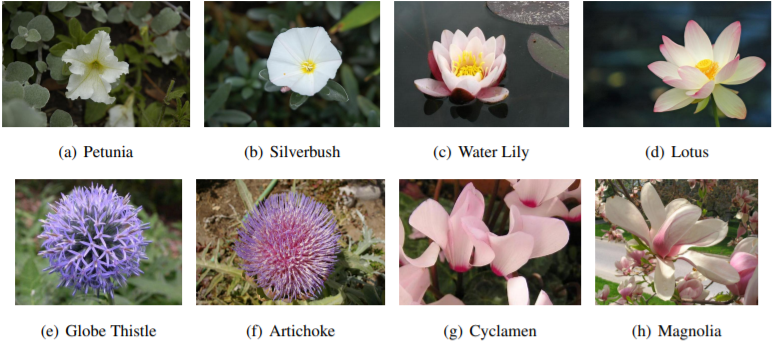
\includegraphics[scale=0.6]{images/flowerclass.PNG}
\caption{Visually similar flower species. As shown in pairs, images from different flower species may even look indistinguishable for non-trained human eyes\textsuperscript{\cite{Oxford}}}
\label{fig:flower similar class}
\end{figure}

\begin{figure}[h!]
\centering
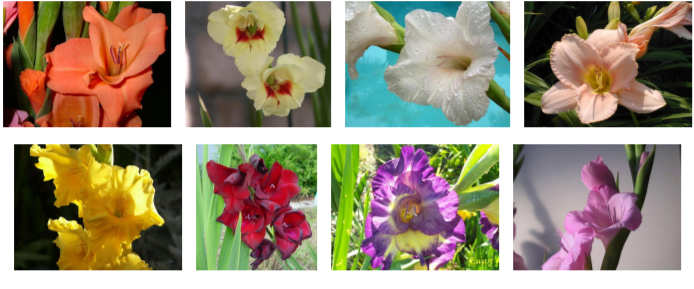
\includegraphics[scale=0.6]{images/disimilar.PNG}
\caption{Visually dissimilar flowers within the same species as shown in the example of sword lily. Sword lilies have a high variation in both color and shape, which makes the recognition problem very challenging \textsuperscript{\cite{Oxford}}}
\label{fig:flower dissimlar class}
\end{figure}


\section{DenseNet}
DenseNet is an extension to Wide Residual Networks. The l\textsuperscript{th} layer has l inputs, consisting of the feature maps of all preceding convolution blocks. Its own feature maps are passed on to all (L-l) subsequent layers. This introduces L(L+1) / 2 connections in an L-layer network, instead of just L, as in traditional feed-forward architectures. Because of its dense connectivity pattern, its referred as Dense Convolution Network \cite{DBLP:journals/corr/HuangLW16a}.
\\It features several improvements such as :

\begin{enumerate}
    \item Dense connectivity : Connecting any layer to any other layer.
    \item Growth Rate parameter : Which dictates how fast the number of features increase as the network becomes deeper.
    \item Consecutive functions : BatchNorm - Relu - Conv which is from the Wide ResNet paper and improvement from the ResNet paper.
\end{enumerate}
The Bottleneck - Compressed DenseNets offer further performance benefits, such as reduced number of parameters, with similar or better performance.

\begin{figure}[h!]
\centering
\includegraphics[scale=0.7]{images/densenet.PNG}
\caption{DenseNet architecture \textsuperscript{\cite{DBLP:journals/corr/HuangLW16a}}}
\label{fig:Densenet}
\end{figure}

\newpage

\section{Training}
\subsection{Pre-Processing}
For the given data set we performed normalisation by resizing the pixel values(0-255) to values ranging between 0-1(float32). We also reshaped the images to pixel range of (128,128).
In order to use data generators more effectively, we have restructured the files in the data set. We then created folders with class labels as their names and saved their respective images to the folder to feed into the model data generator.
Further the test set was made with 20\% of overall dataset which was chosen using a random number counter function.

\subsection{DenseNet}
For the given problem statement, we have modified the DenseNet architecture to get better accuracy in the result. DenseNet architecture has 121 layers, but for our specific model we reduced it into 121/3 layers. The custom Layer of DenseNet used for batch normalization learns a set of weights and biases used for scaling the input data. The output consists simply of an element-wise multiplication of the input and sum of a set of constants:
\newline out = in * gamma + beta,
\newline where 'gamma' and 'beta' are the weights and biases learnt.
Initially we had given learning rate as 0.001 and assigned Plateau to 0.00001 to avoid the local minima.

\subsubsection{Parameter initialisation}
Tensorflow sets certain parameters by default. 
For Conv2D layer the kernel initializer has been set to glorot\_uniform by default. Where as we have set bias to false,since we have made use of the batch normalisation layer which is analogous to bias. 
\newline For Dense layer the kernel initializer is glorot\_uniform.

\newline The easier way of initiatize weight and bias for neural network is to set them to small (perhaps -0.01 to +0.01) uniform random values, which work well with hidden layers but this simple approach may not always work good with deep neural networks especially with ReLu(rectified linear unit) activation function.

\newline One among the common scheme for initialization for deep neural network is Glorot initialization which is also known as Xavier initialization.where we initialize each weight with a small Gaussian value with mean = 0.0 and variance based on the fan-in and fan-out of the weight.
\newline 

\textbf{Custom layer initialization}
\begin{enumerate}
    \item axis=-1
    \item momentum = 0.9
    \item weights=None
    \item beta\_init = zero
    \item gamma\_init = one
\end{enumerate}
\textbf{Arguments}
\begin{enumerate}
     \item Axis: integer, axis along which to normalize in mode 0. For instance,if your input tensor has shape (samples, channels, rows, cols), set axis to 1 to normalize per feature map (channels axis).
       \item momentum: momentum in the computation of the
            exponential average of the mean and standard deviation of the data, for feature-wise normalization.
        \item weights: Initialization weights.List of 2 Numpy arrays, with shapes:[(input\_shape,), (inpu\_shape,)]`
        \item beta\_init: name of initialization function for shift parameter (see [initializations](../initializations.md)), or alternatively,Theano/TensorFlow function to use for weights initialization.This parameter is only relevant if you don't pass a `weights` argument.
        \item gamma\_init: name of initialization function for scale parameter (see
            [initializations](../initializations.md)), or alternatively, Theano/TensorFlow function to use for weights initialization. This parameter is only relevant if you don't pass a `weights` argument.
\end{enumerate}

       


\subsection{Augmentation}
To improve the data set size, we choose data augmentation methods. Parameter for data augmentation for images are as follows:
\newline rotation range=90,width shift range=0.1,height shift range=0.1,zoom range=0.2,re scale = 1/255,horizontal flip = True,vertical flip = True,validation split=0.22,fill mode = 'nearest'(Points outside the boundaries of the input are filled according to the given mode). Please note that data augmentation is only cared out the train dataset but not to test dataset which is split before any augmentation.

\begin{figure}[h!]
\centering
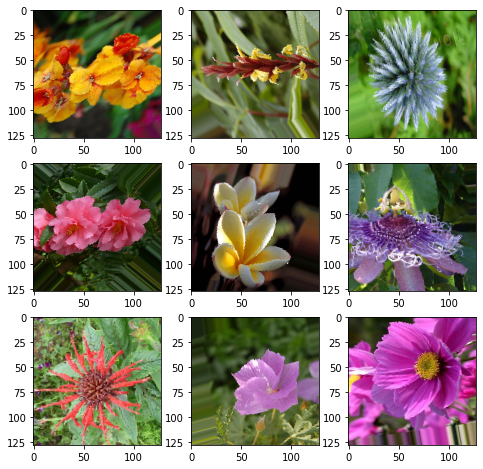
\includegraphics[scale=0.6]{images/download.png}
\caption{Example for augmented images}
\label{fig:Results}
\end{figure}

\subsection{Hyper parameter tuning}
Model optimisation is one of the toughest part in deep learning algorithms. We have used different parameters to test and modify the model for the greater good of performance and accuracy.
We tuned on learning rate, number of epochs and Convolution Kernel Width. We also added callbacks while training for model weight saving when model improves, for saving training evaluations in a csv files, for early stopping which monitors val\_loss and stopped training to 120 epochs

\section{Results}

The main goal of the task was to classify 102 classes of data set with maximum accuracy. We have used DenseNet architecture as a classification approach to provide the solution to the problem.
On our first check point of the model, we got the results as given in figure 4(results without hyper-parameter tuning):

\begin{figure}[h!]
\centering
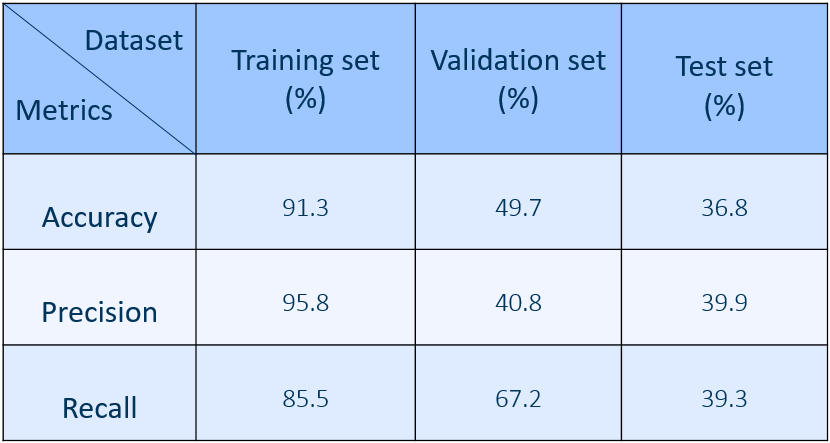
\includegraphics[scale=0.7]{images/Capture.PNG}
\caption{Overall Results without hyper-parameter tuning}
\label{fig:Results}
\end{figure}

We can see from the results that our model is overfitted.
In order to reduce the overfitting, we incorporated augmentation and regularization methods.
We introduced dropout layers at dropout rate =0.5, batch normalisation and weight decay(L2 regularization).
We have increased the number of epochs to 200 in order to ensure the stability of accuracy but due to early stopping callback we only got 120 epochs training. 

After remedies to over-fitting and hyper parameter tuning, our final results are as shown in figure 5(results after hyper-parameter tuning):

\begin{figure}[h!]
\centering
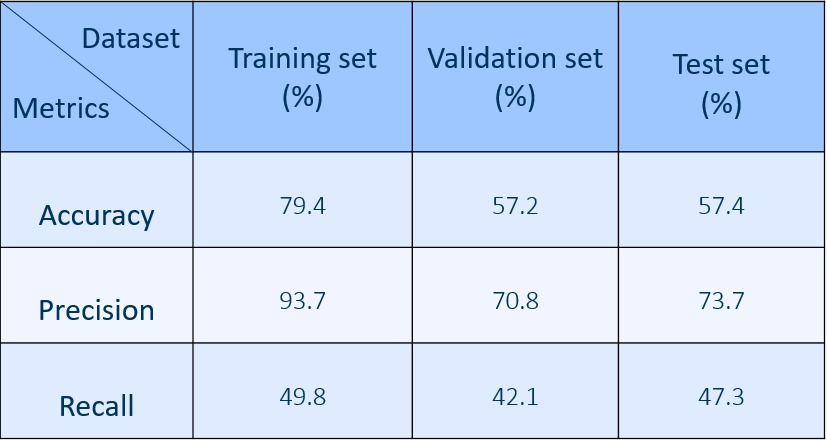
\includegraphics[scale=0.45]{images/Results_after.jpeg}
\caption{Overall Results after hyper-parameter tuning}
\label{fig:Results}
\end{figure}

\subsection{Accuracy over each class}
As seen in Fig.8, we have plotted percentage accuracy over the 102 classes of the dataset showing clear picture of the classes which have overall class results.

From the graph we can interpret that class 20, class 100 and class 29 are giving 0\% accuracy over test set. Hence we consider them as worst classifications.
In order to inspect the problem of worst classification,below are some of the examples representing classes with accuracy of zero percentage.

We assume that from the examples,wide variations in texture, size and number of flowers in the image maybe the parameters which didn't allow the model to learn the classification accurately.

The average of over all class specific results is 56.6\% which is very near to the overall results of test set i.e.57.4\%




\begin{figure}[!htb]
\minipage{0.32\textwidth}
  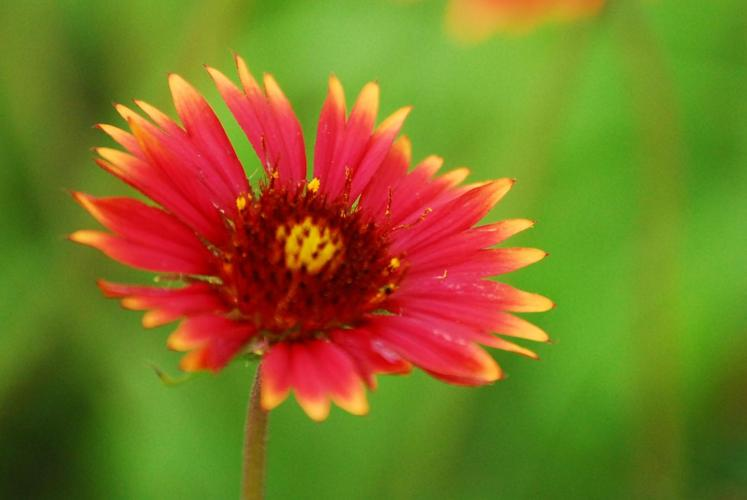
\includegraphics[width=5cm, height=5cm]{images/image_07933.jpg}
  \caption{Class 100(training)}\label{fig:awesome_image1}
\endminipage\hfill
\minipage{0.32\textwidth}
  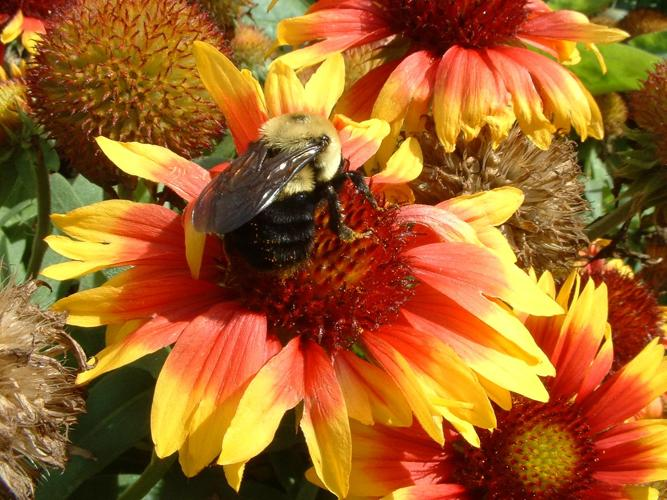
\includegraphics[width=5cm, height=5cm]{images/Class100_1.jpg}
  \caption{Class 100(test)}\label{fig:awesome_image2}
\endminipage\hfill
\minipage{0.32\textwidth}%
  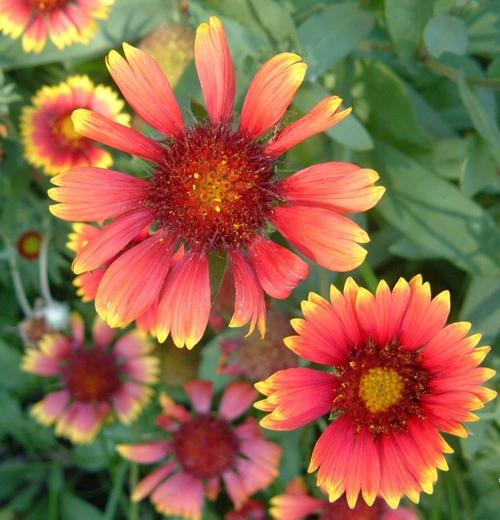
\includegraphics[width=5cm, height=5cm]{images/Class100_2.jpg}
  \caption{Class 100(test)}\label{fig:awesome_image3}
\endminipage
\end{figure}




\begin{figure}[!htb]
\minipage{0.32\textwidth}
  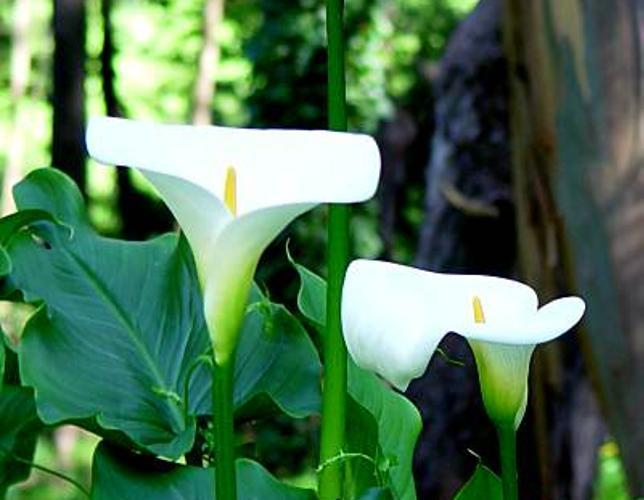
\includegraphics[width=5cm, height=5cm]{images/image_04923.jpg}
  \caption{Class 20(training)}\label{fig:awesome_image1}
\endminipage\hfill
\minipage{0.32\textwidth}
  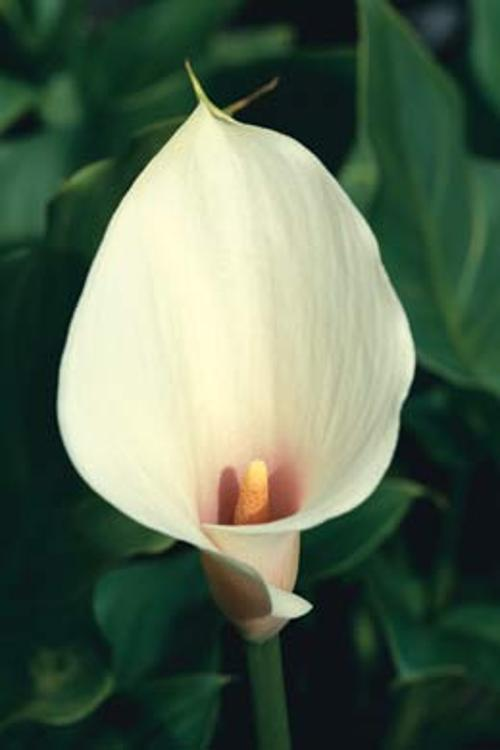
\includegraphics[width=5cm, height=5cm]{images/Class20_2.jpg}
  \caption{Class 20(test)}\label{fig:awesome_image2}
\endminipage\hfill
\minipage{0.32\textwidth}%
  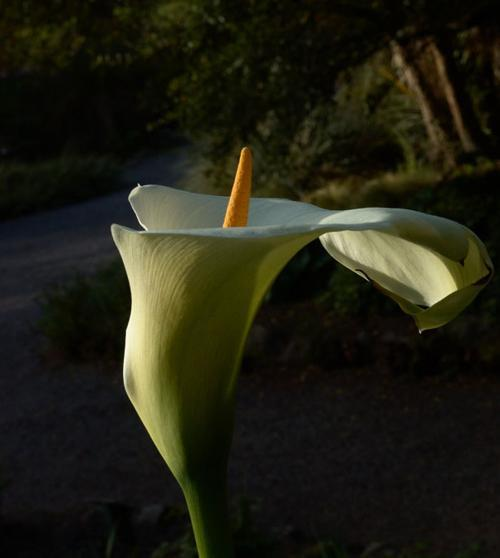
\includegraphics[width=5cm, height=5cm]{images/Class20_3.jpg}
  \caption{Class 20(test)}\label{fig:awesome_image3}
\endminipage
\end{figure}





\begin{figure}[h!]
\centering
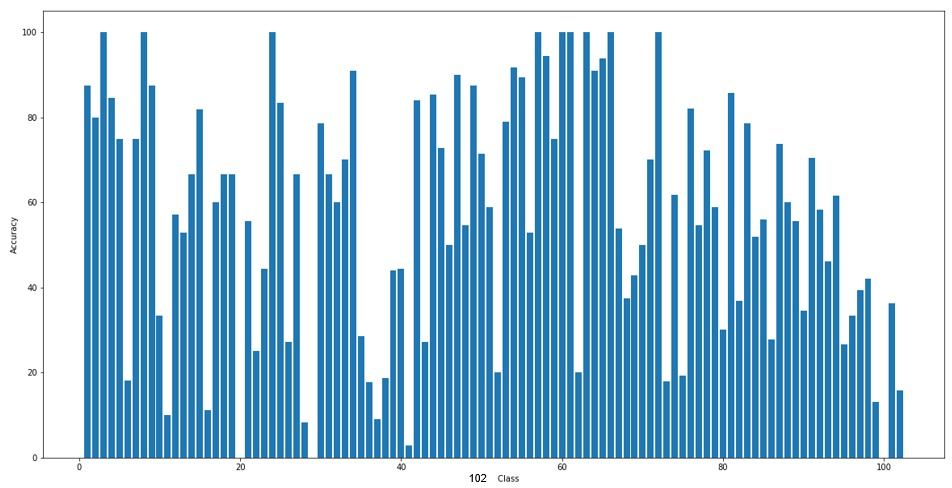
\includegraphics[scale=0.4]{images/Acc_Each_Class.png}
\caption{Accuracy over Each Class}
\label{fig:Results}
\end{figure}

\begin{figure}[h!]
\centering
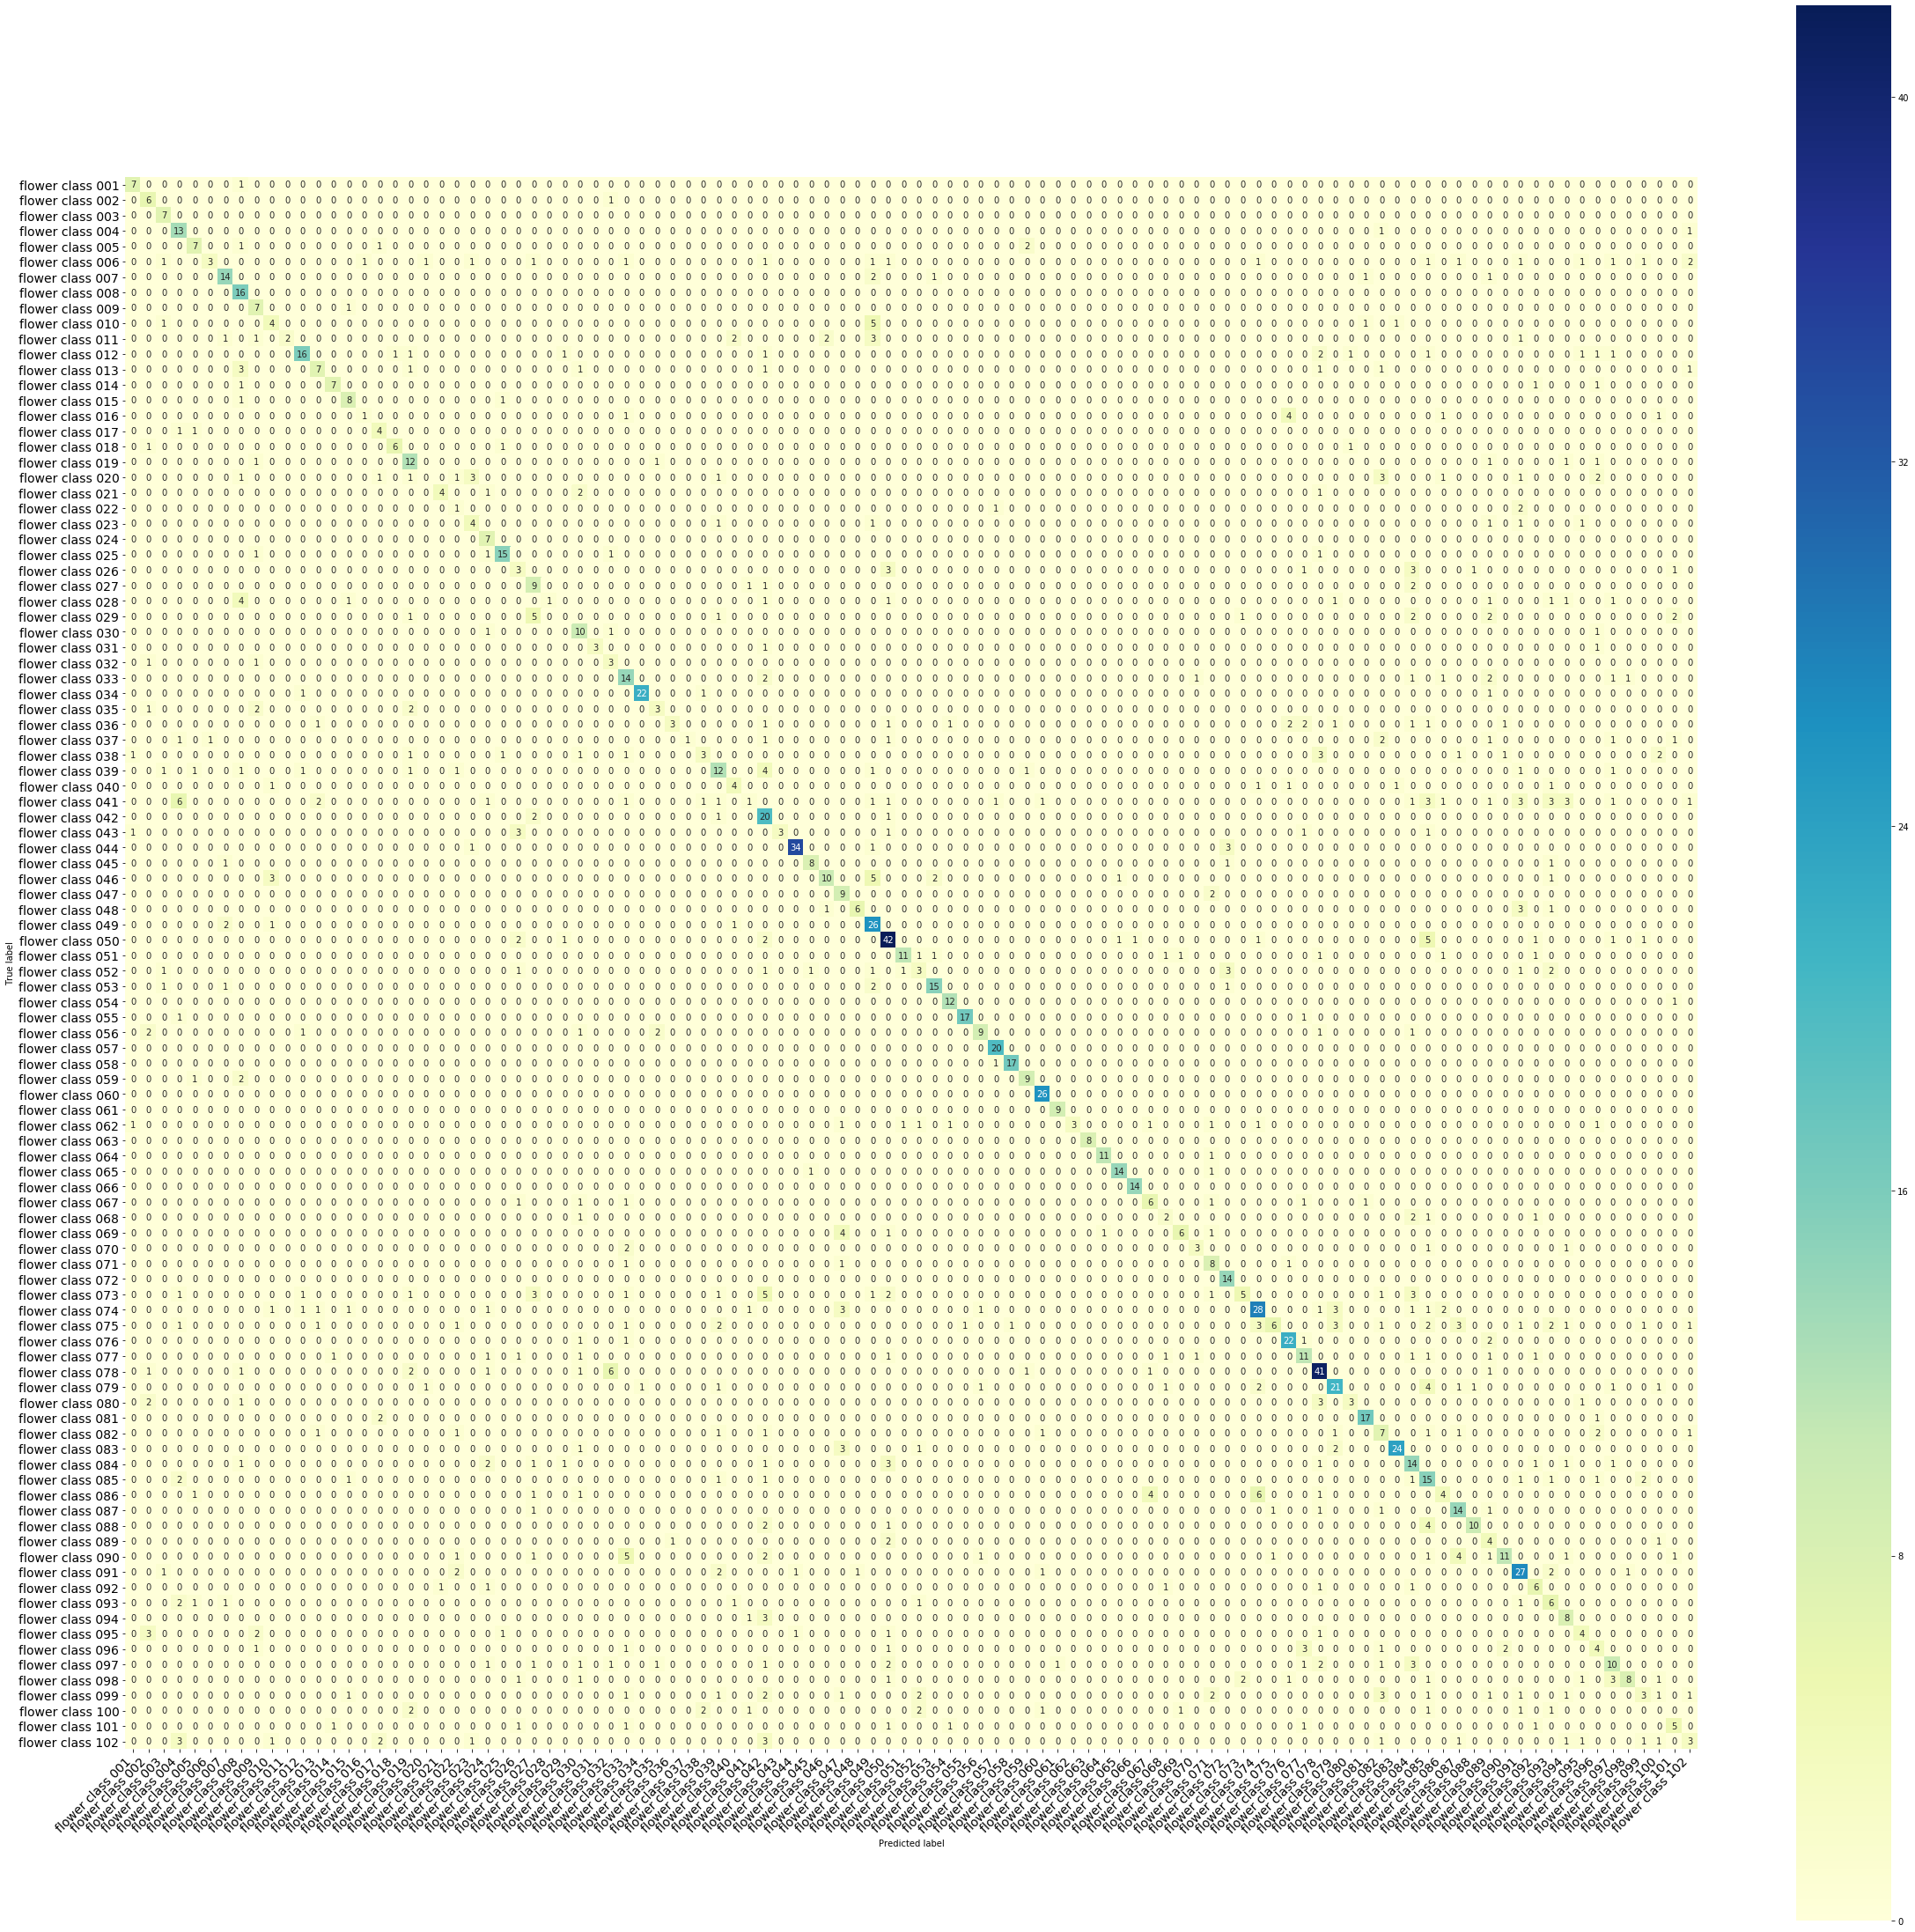
\includegraphics[scale=0.225]{images/heatmaps.png}
\caption{Confusion matrix as a heatmap}
\label{fig:Results}
\end{figure}


\subsection{Evaluation Results} 

\begin{figure}[h!]
\centering
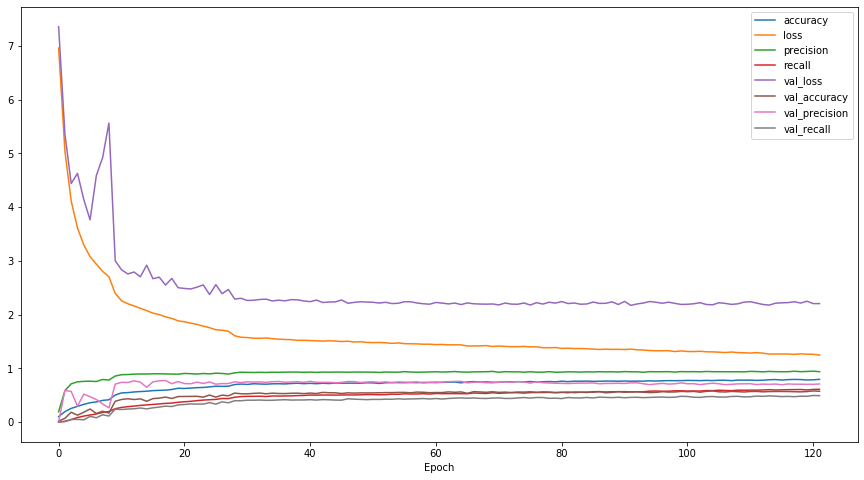
\includegraphics[scale=0.6]{images/overalleva.png}
\caption{Evaluation Results}
\label{fig:Results}
\end{figure}

From the evaluation results plot(Figure 6), we can clearly see there is no substantial variations after 25 epochs, but we chose to run our model up to 120 epochs in order to make sure the consistency of results. 


\subsubsection{Area under curve}

In order to better interpret our idea on label imbalance which is present in our data-set, we chose to plot precision vs recall curve(figure 7 and Figure 8).


\begin{figure}[h!]
  \centering
  \begin{minipage}[b]{0.4\textwidth}
    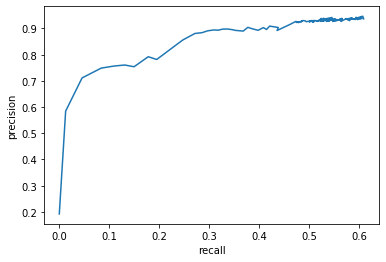
\includegraphics[scale=0.6]{images/aoct.png}
    \caption{Area Under Curve}
    \label{fig:Area Under Curve}
  \end{minipage}
  \hfill
  \begin{minipage}[b]{0.4\textwidth}
    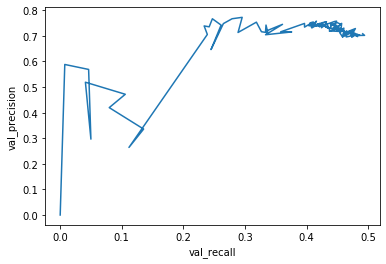
\includegraphics[scale=0.6]{images/aocv.png}
    \caption{Area Under Curve for Validation Set}
    \label{fig:Area Under Curve for Validation Set}
  \end{minipage}
\end{figure}


\subsubsection{Accuracy plot}

\begin{figure}[h!]
\centering
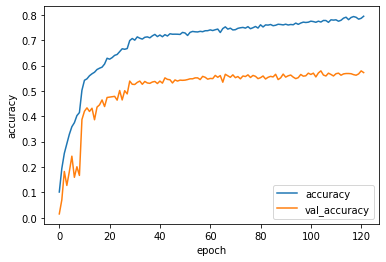
\includegraphics[scale=0.7]{images/acc.png}
\caption{Accuracy}
\label{fig:Accuracy}
\end{figure}

This graph indicates the accuracy of model over number of epochs for training and validation data set. As we can see from the graph, after 25 epochs there is no much improvement in learning.Irrespective of learning process, we extended our epoch to 120 to make sure the certainty of the results.


\subsubsection{Recall and precision plots}
recall refers to the percentage of total relevant results correctly classified by your algorithm. Precision means the percentage of your results which are relevant.
The following curve indicate the recall over each epoch(fig.18) and precision over each epoch(fig.19)

\begin{figure}[h!]
  \centering
  \begin{minipage}[b]{0.4\textwidth}
    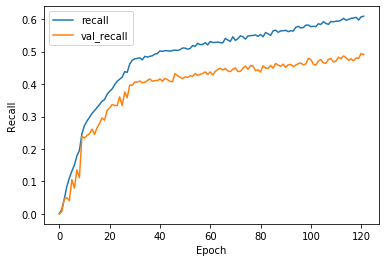
\includegraphics[scale=0.6]{images/re.png}
    \caption{Recall}
    \label{fig:Recall}
  \end{minipage}
  \hfill
  \begin{minipage}[b]{0.4\textwidth}
    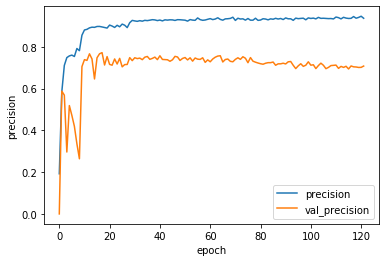
\includegraphics[scale=0.6]{images/pre.png}
    \caption{Precision}
    \label{fig:Precision}
  \end{minipage}
\end{figure}

\section{Conclusion}
We do believe in exploring and exploiting the state-of-the-art technology and hence we tackled the problem statement with DenseNet implementation. To our best of knowledge, we made modifications to DenseNet architecture in order to solve our problem statement.The size of our data set can be one of the major limitations for the performance of our model. We handled this problem with the technique of data augmentation as mentioned earlier. This was an addition to the improvement in our results with the help of hyper-parameter tuning and techniques to tackle over-fitting, which in turn increased the accuracy of our model. 
We believe that further gains in accuracy of DenseNets may be obtained by more detailed tuning of hyper-parameters and customization in DenseNet architecture.

\subsection{GitHub link for source code}
Please find the link for source code hosted in GitHub at 
\href{https://github.com/785pavan/FlowerClassfication}{https://github.com/785pavan/FlowerClassfication}\footnote{https://github.com/785pavan/FlowerClassfication}. The latest iteration of our model is mark08 and you can even find h5 files for using this for transfer learning if needed.





\bibliographystyle{plain}
\newpage
\bibliography{references}






\end{document}
